\section{Case study}
\label{sec:case_study}

\subsection{Actors and physical setup}

\Cref{fig:setup-scheduling}a shows the setup. Heat producers operate CHP plants, waste incineration plants, heat pumps and peak boilers. VEKS buys heat from the producers under heat purchase agreements, transports it through its transmission network and sells it to local distribution companies under heat delivery agreements. Varmelast coordinates production planning across the interconnected system on behalf of VEKS, CTR and HOFOR~\cite{varmelast_dispatch}. HTF receives heat from VEKS through a heat-exchanger station, adds local production from two heat pumps and distributes the heat to customers in Taastrup and Hedehusene.

The PTES is jointly owned by VEKS and HTF, each holding 50\%, and VEKS holds the right to use HTF's share against an annual compensation~\cite{planenergi_hoje_taastrup}. The storage is charged from the transmission line and discharged into HTF's network, where the discharged heat replaces direct supply through the heat exchanger. It stores sensible heat in a stratified water volume (\cref{fig:modes-of-operation}) and was designed for short-term operation with cycles of one to two weeks rather than for seasonal storage~\cite{sifnaios2025performance}.

\begin{figure}[!htb]
    \centering
    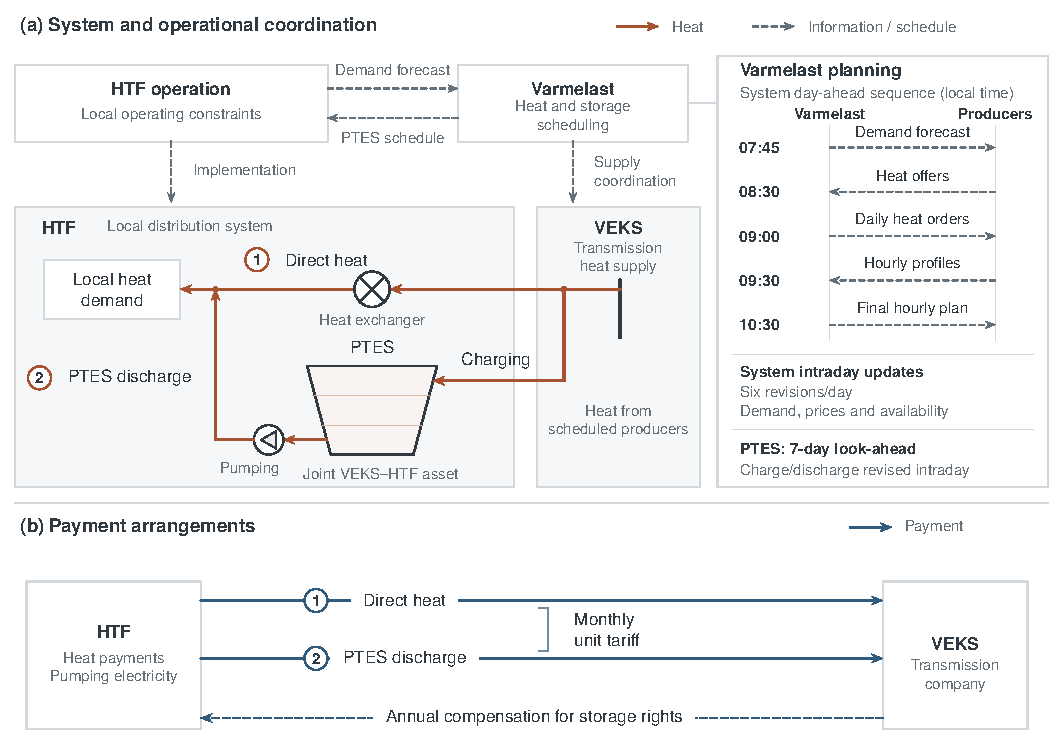
\includegraphics[width=\linewidth]{figures/ptes_setup_and_scheduling.pdf}
    \caption{Høje Taastrup PTES in the Copenhagen district heating system. (a) Heat flows, information exchange and the day-ahead planning sequence of Varmelast. (b) Current payment arrangement between HTF and VEKS: direct heat (1) and PTES discharge (2) are billed at the same monthly tariff, HTF bears the pumping electricity for discharge, and VEKS pays an annual compensation for the storage rights.}
    \label{fig:setup-scheduling}
\end{figure}

\begin{figure}[!htb]
    \centering
    \begin{subfigure}[b]{0.45\linewidth}
        \centering
        \resizebox{\linewidth}{!}{\inputtikzfigure{figures/charge_body}}
        \caption{Charging: upper inlet, lower outlet.}
        \label{fig:modes-of-operation-charge}
    \end{subfigure}
    \hfill
    \begin{subfigure}[b]{0.45\linewidth}
        \centering
        \resizebox{\linewidth}{!}{\inputtikzfigure{figures/discharge_body}}
        \caption{Discharging: upper outlet, lower inlet.}
        \label{fig:modes-of-operation-discharge-1}
    \end{subfigure}
    \caption{Conventional PTES charging and discharging. Configurations using the middle connection are omitted.}
    \label{fig:modes-of-operation}
\end{figure}

\subsection{Scheduling and settlement}

Varmelast dispatches production by variable cost, accounting for the electricity revenue of CHP plants, so that the net cost of heat can be low or even negative when electricity prices are high~\cite{varmelast_dispatch}. A coordinated day-ahead heat plan is published at 10:30 and revised six times per day (\cref{fig:setup-scheduling}a). Varmelast has scheduled the PTES since January 2024, initially with a 24-hour horizon and from late 2024 with a seven-day horizon~\cite{sifnaios2025performance}.

Dispatch costs and settlement prices are separate. VEKS pays producers under producer-specific agreements, and distribution companies pay a monthly tariff for transmission heat~\cite{varmelast_local_production}. HTF pays the same monthly tariff for direct heat and for heat discharged from the PTES, and pays the pumping electricity required for discharge (\cref{fig:setup-scheduling}b). Under this arrangement, replacing direct supply by scheduled discharge does not reduce HTF's heat payment but increases its electricity cost. The system value of discharging at the scheduled times therefore does not reach the party that implements it. The annual compensation remunerates the storage capacity, not its use.
